\documentclass[journal]{IEEEtran}
\usepackage[hidelinks]{hyperref}
\usepackage{graphicx}

\begin{document}

\title{The Use of Quantum Computing\\ in Algorithmic Trading}

\author{Paulina~Brzecka,
        Marek~Borzyszkowski,
        Wojciech~Baranowski
        and~Piotr~Mironowicz%
\thanks{P. Brzecka, M. Borzyszkowski and W. Baranowski were with the Faculty 
of Electronics, Telecommunications and Informatics, Gdansk University of Technology, Gdansk,
Poland.}%
\thanks{P. Mironowicz, the project mentor, was with the Faculty 
of Electronics, Telecommunications and Informatics, Gdansk University of Technology, Gdansk,
Poland.}
}

\markboth{Journal of \LaTeX\ Class Files,~Vol.~14, No.~8, December~2024}%
{The Use of Quantum Computing\\ in Algorithmic Trading}

\maketitle

\begin{abstract}
Algorithmic trading is an investment strategy that leverages automated systems to make decisions in financial markets. Quantum computing presents opportunities to enhance these strategies by processing market data and analyzing trends with greater efficiency. This research explores implementing an agent utilizing quantum computing to make investment decisions in the stock market. The agent is evaluated using both quantum computer emulators and physical quantum hardware, comparing its performance to classical algorithms. Preliminary results show potential advantages in prediction quality and resource utilization, paving the way for further studies in quantum-enhanced financial strategies.
\end{abstract}

\begin{IEEEkeywords}
Algorithmic trading, investing, trading systems, financial markets, Quantum computing, market predicting.
\end{IEEEkeywords}

\section{Introduction}
Algorithmic trading has revolutionized the landscape of financial markets, significantly altering the way investment decisions are made. By employing automated trading systems, algorithmic trading allows for rapid execution of trades, often within fractions of a second, based on predefined strategies and market conditions. This ability to process vast amounts of data and make instantaneous decisions has proven to be highly effective in capturing market opportunities. However, as financial markets grow increasingly complex, traditional computational methods often struggle to keep up with the scale and intricacy of market data. The exponential increase in data volume, the need for real-time processing, and the high-dimensionality of the data pose significant challenges for classical algorithms.

Quantum computing, on the other hand, offers a promising alternative. By leveraging quantum bits (qubits) and the principles of superposition and entanglement, quantum computers can process information in parallel, potentially solving problems that are intractable for classical computers. Quantum algorithms are designed to take advantage of these quantum mechanical properties, offering the potential for faster data processing and more efficient problem-solving in areas such as optimization, simulation, and machine learning. In particular, quantum computing could address some of the limitations faced by classical computational methods in the context of algorithmic trading, where the need for speed, accuracy, and efficiency is paramount.

This paper aims to investigate the implementation and evaluation of both classical and quantum algorithms for stock market prediction, with a focus on predicting asset prices based on historical data. While classical algorithms, such as Principal Component Analysis (PCA) and Support Vector Machines (SVM), are well-established and widely used in various financial applications, their quantum counterparts—Quantum Principal Component Analysis (QPCA) and Quantum Support Vector Machines (QSVM)—remain underexplored in the context of financial market predictions. The research presented in this paper seeks to fill this gap by conducting a comparative analysis of the performance of classical and quantum algorithms in a controlled environment. By exploring how these algorithms perform on historical stock market data, the paper aims to shed light on the potential advantages and challenges of incorporating quantum computing into the field of algorithmic trading.

\section{Algorithms Overview}
\subsection{Principal Component Analysis (PCA)}
Principal Component Analysis (PCA) \cite{pca} is a widely-used dimensionality reduction technique that allows for the simplification of complex datasets while retaining as much of the variance as possible. The goal of PCA is to transform a dataset into a new coordinate system, where the axes (known as principal components) correspond to the directions of maximum variance in the data. By projecting data onto a lower-dimensional space, PCA reduces the number of features needed to represent the data, making it easier to analyze and visualize. This process is particularly useful in fields such as finance, where large amounts of historical market data may include redundant or highly correlated features.

The strength of PCA lies in its ability to identify patterns in data and eliminate noise, making it a powerful tool for preprocessing in machine learning models. In the context of stock market prediction, PCA can be applied to identify key factors that drive asset prices and reduce the dimensionality of market data, thereby simplifying the problem and improving the performance of subsequent predictive models. However, while PCA is effective in capturing linear relationships in data, it may struggle to identify more complex, nonlinear patterns that are often present in financial markets. This limitation has driven the development of more sophisticated algorithms, including those that leverage quantum computing.

\subsection{Support Vector Machines (SVM)}
Support Vector Machines (SVMs) \cite{svm} are a class of supervised learning algorithms primarily used for classification and regression tasks. The main idea behind SVM is to find the optimal hyperplane that best separates data points belonging to different classes or, in the case of regression, fits the data with minimal error. In its simplest form, SVM constructs a hyperplane in a high-dimensional space that maximizes the margin between two classes. For regression tasks, SVM aims to find a function that has the smallest deviation from the actual data points within a predefined margin of tolerance.

SVM is particularly effective when dealing with high-dimensional data, such as in financial markets, where the number of input features can be very large. SVM's ability to work well in such high-dimensional spaces makes it a valuable tool for stock market prediction, where features such as historical prices, trading volume, and various technical indicators may serve as inputs to the model. However, SVM's effectiveness can be limited by the choice of kernel and the computational complexity associated with training the model, particularly when dealing with large datasets or a high number of support vectors. These challenges highlight the potential for improvement through quantum-enhanced algorithms, which may offer solutions to speed up the training process and improve model performance.

\subsection{Quantum Principal Component Analysis (QPCA)}
Quantum Principal Component Analysis (QPCA) \cite{qpca} is an extension of classical PCA that leverages quantum mechanics to accelerate the process of dimensionality reduction. The basic principle behind QPCA is to use quantum superposition and entanglement to perform linear algebra operations in parallel, which can significantly reduce the computational time required to analyze large datasets. While classical PCA typically requires matrix diagonalization, a process that grows increasingly complex as the size of the data increases, QPCA uses quantum states to encode and process the data in a way that allows for exponential speedup under certain conditions.

In the context of stock market prediction, QPCA holds the potential to analyze large datasets more efficiently than classical PCA. The ability to handle high-dimensional data with quantum speedup could enable quicker identification of key features that influence asset prices, leading to more effective predictive models. However, implementing QPCA in practice remains challenging due to the limited availability of quantum hardware and the need for specialized quantum algorithms that can be applied to real-world financial data. Nonetheless, QPCA represents a promising direction for quantum-enhanced data analysis, with the potential to transform how financial markets are analyzed and predicted.

\subsection{Quantum Support Vector Machines (QSVM)}
Quantum Support Vector Machines (QSVM) \cite{qsvm} are an adaptation of classical SVM algorithms designed to take advantage of quantum computing's unique capabilities. While traditional SVM relies on kernel functions to map input data into a higher-dimensional space, QSVM utilizes quantum kernels that are based on quantum states, allowing the model to operate in exponentially larger feature spaces. This enables QSVM to capture more complex, nonlinear relationships in data, which is especially important in the context of stock market prediction, where relationships between features can be highly intricate and non-linear.

QSVM operates by encoding data into quantum states, applying quantum kernels to calculate the inner products between these states, and then using these results to find the optimal hyperplane for classification or regression tasks. The key advantage of QSVM over classical SVM is the potential for exponential speedup in terms of both the time required for training and the model's ability to handle larger datasets. For stock market prediction, QSVM can be particularly useful in situations where classical algorithms struggle to capture the complexities of market dynamics. However, the practical implementation of QSVM is still in its early stages, and significant challenges remain in terms of developing quantum hardware and algorithms that can handle the scale and noise associated with financial data.

\section{Methodology}
\subsection{Data Collection}

The first step in the research process was the collection of historical stock market data. To ensure the breadth of market trends, data was gathered from index S\&P 500, representing 500 of the largest companies in the United States. This selection allows for the comparison of data from developed markets, providing a reliable set of inputs for the algorithm training and testing phases.

The data spans from the beginning of 2003 to the end of 2023, offering a long-term perspective on market behavior. The dataset includes not only the daily closing prices of the individual companies but also the indices themselves, providing a broader context for understanding the behavior of the stock prices in relation to the overall market. For each day of trading, the dataset includes essential fields such as the date, opening price, highest and lowest price reached during the session, the closing price, and the trading volume. These features are critical for analyzing the movement of asset prices and understanding the broader market dynamics.

Additionally, the dataset includes information on market capitalization and sector performance, allowing the models to take into account various factors that influence asset price fluctuations. This comprehensive set of features ensures that the prediction models can consider both individual asset performance and market-wide trends.

The data was stored in CSV format for ease of processing and manipulation. Preprocessing steps involved cleaning the data by handling missing values, removing outliers, and normalizing the features to ensure comparability across all variables. This process helped prepare the data for the training phase, ensuring high-quality input that would minimize potential noise and increase the accuracy of the predictive models.

\subsection{Experiment Design}
The core objective of the experiment was to evaluate the performance of both classical and quantum algorithms in predicting stock market prices. The focus was placed on forecasting the closing price of an asset based on the closing prices from the previous five days, as this approach has been shown to capture enough historical context for accurate predictions in financial markets.

The dataset was divided into training and test sets, with 2/3 of the data used for training and the remaining 1/3 reserved for testing. This training-test split is a commonly used approach in machine learning experiments, ensuring that the models are both adequately trained and evaluated on unseen data. The training data consisted of fourteen years of stock market data, while the test data covered the following seven years. This separation of training and testing periods helps ensure that the algorithms are evaluated on out-of-sample data, mimicking real-world conditions where future data is unknown during model training.

For each algorithm, the training set was used to teach the model how to predict the closing price of a given asset based on the historical data. The model was then evaluated on the test set to assess its predictive accuracy, with performance metrics such as mean absolute error (MAE) and root mean squared error (RMSE) used to quantify the error between predicted and actual closing prices.

\subsection{Implementation}

The implementation of the algorithms involved the application of both classical and quantum machine learning techniques.

\begin{itemize}
    \item \textbf{Principal Component Analysis (PCA)} was implemented using popular Python libraries such as scikit-learn. PCA was employed as a preprocessing step to reduce the dimensionality of the data, capturing the most significant features while discarding less important ones. The reduced dataset was then used as input for subsequent machine learning models, improving the efficiency and effectiveness of training.
    \item \textbf{Support Vector Machines (SVM)} were implemented using the scikit-learn library. SVM is a powerful algorithm for both classification and regression, and it was employed to model the relationship between the features extracted by PCA and the closing prices of assets. Different kernel functions (linear, radial basis function) were tested to identify the most suitable kernel for predicting stock prices.
\end{itemize}

\begin{itemize}
    \item \textbf{Quantum Principal Component Analysis (QPCA)} was implemented using the Qiskit framework, an open-source quantum computing library. QPCA was used as an alternative to classical PCA, leveraging quantum operations to process data exponentially faster in certain conditions. However, the quantum version of PCA was tested only on quantum computer simulators, as access to actual quantum hardware was not available for this experiment. The simulator allowed us to test the algorithm’s scalability and efficiency under various configurations.
    \item \textbf{Quantum Support Vector Machines (QSVM)} were implemented using Qiskit as well. QSVM applies quantum computing techniques to enhance the SVM model by using quantum kernels, which map data points into higher-dimensional feature spaces, enabling the model to capture more complex patterns. Similar to QPCA, QSVM was also tested solely on quantum simulators, as real quantum hardware was not utilized during the experiment.
\end{itemize}

Each algorithm was tested and optimized using cross-validation techniques to tune hyperparameters, ensuring that the models are generalized and avoid overfitting to the training data. The final models were then evaluated on the test set to assess their performance in predicting unseen data.

\subsection{Hardware Specifications}

The experiments were carried out on a local computing system with the following specifications:

\begin{itemize}
    \item \textbf{CPU}: Intel Core i5-4590, a quad-core processor running at 3.3 GHz, providing solid computational power for the training of both classical and quantum models.
    \item \textbf{RAM}: 32 GB DDR3 1600Hz, sufficient for handling the large datasets required for the training of machine learning models, especially when working with multiple features and time-series data.
    \item \textbf{Swap}: 512 GB, serving as an extended memory to handle large datasets and prevent system crashes during memory-intensive operations.
    \item \textbf{Storage}: WD 2TB M.2 PCIe Gen4 NVMe Black SN770, providing high-speed storage with a high throughput, essential for reading and writing large datasets efficiently.
\end{itemize}

For the quantum algorithms, experiments were run on quantum simulators, which were used to simulate quantum computing behavior on a classical computer. These simulators allowed the evaluation of QPCA and QSVM without the need for actual quantum hardware. The use of quantum simulators enabled testing and performance analysis under different configurations, but the results are not directly representative of how the algorithms would perform on real quantum devices.

For classical algorithms, all training and testing were conducted on the local system, which provided a controlled environment for performance comparison between classical and quantum-based methods.

\section{Results for predictions}

\subsection{Predicted Price vs. Actual Price}

Figure~\ref{fig:price_comparison} illustrates the predicted closing prices of the S\&P 500 index using PCA, SVM, QPCA, and QSVM models compared to the actual values during the test period (2017--2024). The results highlight substantial differences in the predictive accuracy and adaptability of these approaches.

\textbf{PCA:} The PCA predictions maintain a strong correlation with the true price movements, albeit with a consistent lag of 1--2 days. This delay becomes particularly evident during periods of heightened market volatility, where abrupt price changes cause temporary deviations. However, outside of these volatile phases, PCA exhibits robust accuracy, aligning closely with the true market trends.

\textbf{SVM:} SVM predictions show significant divergence from the actual price trends. The model fails to generalize well, likely due to overfitting during training. Consequently, its predictions deviate erratically, rendering it ineffective for continuous market prediction tasks. However, in the case of individual stock predictions (e.g., Meta or Chevron Corp), the SVM model demonstrates the ability to make accurate forecasts as long as the stock trends remain similar to those encountered during training (figure ~\ref{fig:cvx_svm}). Once an unprecedented market trend emerges, the model's performance deteriorates rapidly, highlighting its inability to adapt to new patterns.

\textbf{QPCA:} The QPCA model fails to effectively capture market dynamics, producing predictions that remain largely static over time. This lack of responsiveness results in predictions that do not reflect actual price movements or trends. While the quantum-enhanced approach theoretically offers potential, its current implementation does not provide practical advantages over classical methods, particularly given its substantial computational resource requirements.

\textbf{QSVM:} QSVM predictions exhibit the most considerable deviations among all models. Despite the theoretical advantages of quantum computing, the QSVM struggles with noise and the inherent complexity of financial data. The resulting predictions often fail to align with the overall trend, further amplifying the resource demands of the quantum approach.

The comparison underscores that classical PCA remains the most reliable method among the tested algorithms, while the quantum models (QPCA and QSVM) require further refinement to match their theoretical potential in real-world applications.

\begin{figure}[ht!]
    \centering
    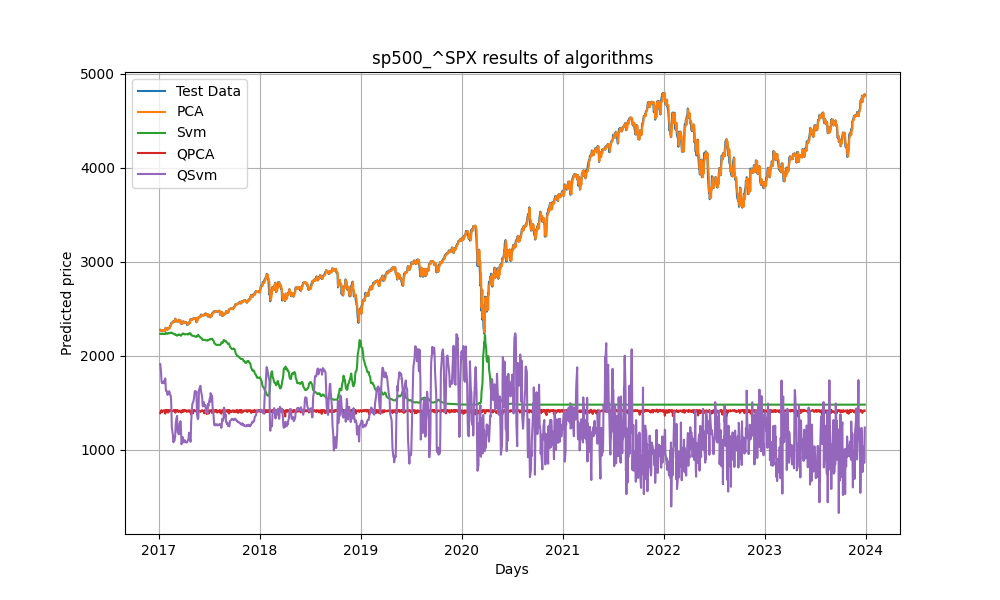
\includegraphics[width=\linewidth]{predicted_vs_actual_price.png}
    \caption{Predicted prices vs. actual prices for the S\&P 500 index.}
    \label{fig:price_comparison}
\end{figure}

\begin{figure}[ht!]
    \centering
    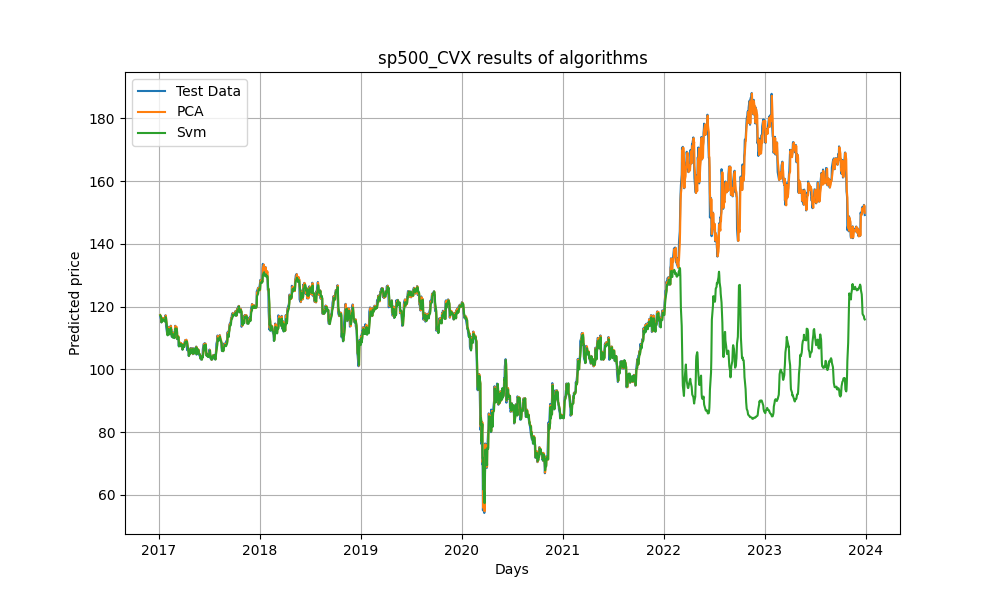
\includegraphics[width=\linewidth]{cvx_svm.png}
    \caption{Predicted prices vs. actual prices for the Chevron Corp stock.}
    \label{fig:cvx_svm}
\end{figure}

\subsection{Prediction Error vs. Time}

Figure~\ref{fig:error_comparison} illustrates the absolute prediction errors over time for PCA, SVM, QPCA, and QSVM models. The analysis highlights significant differences in the error behavior across the algorithms.

\textbf{PCA:} PCA exhibits consistently low prediction errors, with occasional spikes during periods of heightened market volatility. These spikes align with sharp deviations in predicted prices, indicating that PCA's sensitivity to sudden market movements contributes to temporary increases in error. Despite these spikes, PCA demonstrates overall reliability, maintaining low errors throughout the test period.

\textbf{SVM:} SVM consistently produces large prediction errors, reflecting its struggles to generalize from training data to unseen market conditions. The magnitude and persistence of these errors confirm the model’s inadequacy for capturing the dynamic patterns of stock market behavior. However, for individual stocks, the prediction error was relatively small as long as the stock trends remained consistent with those observed during training. Once the model encountered an unfamiliar market trend, the error increased significantly, further emphasizing its limitations in adapting to new scenarios.


\textbf{QPCA:} QPCA demonstrates error behavior that is comparable to majority of SVM results. While the errors are not as erratic as those of QSVM, they remain significant and follow a similar pattern to SVM, indicating that QPCA also struggles to generalize effectively and adapt to dynamic market conditions.

\textbf{QSVM:} QSVM demonstrates erratic and highly variable prediction errors, particularly during periods of market volatility. The model's sensitivity to noise and its computational challenges result in significant deviations from actual values. Consequently, QSVM errors are not only larger but also less predictable compared to the other models.

The comparison underscores that PCA offers the most consistent and reliable performance among the tested algorithms, while SVM, QPCA, and QSVM face critical challenges in predicting stock market behavior accurately.


\begin{figure}[ht!]
    \centering
    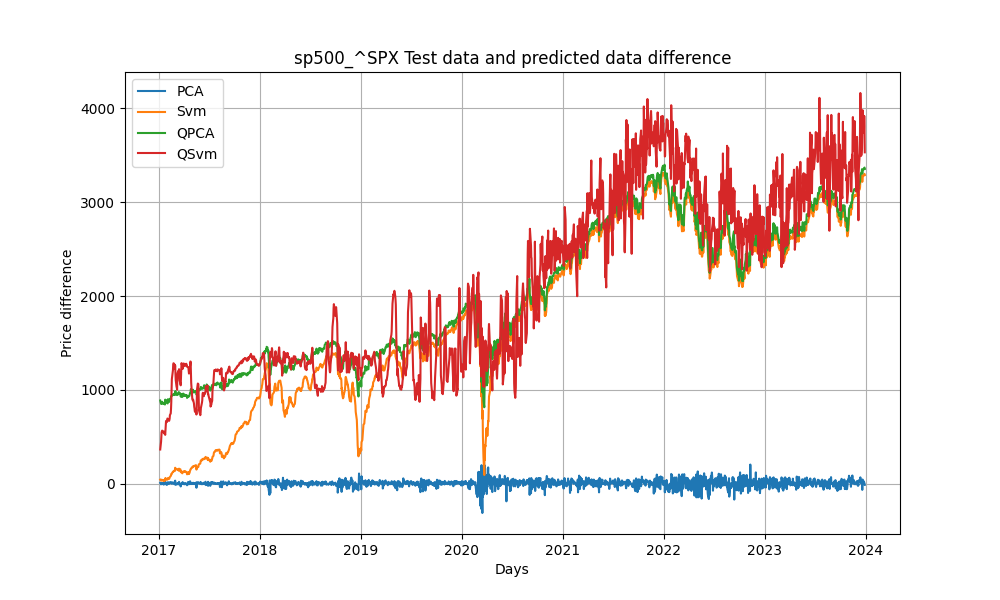
\includegraphics[width=\linewidth]{prediction_error.png}
    \caption{Prediction errors over time for PCA and SVM.}
    \label{fig:error_comparison}
\end{figure}

\subsection{Error Metrics}

The performance of PCA and SVM was also evaluated using several error metrics, which are summarized in Table I. The results confirm the visual observations, with PCA showing significantly lower error values across all metrics, indicating its strong ability to predict the S\&P 500 index’s price movements. In contrast, SVM demonstrates large prediction errors, which suggest that it is less effective for this particular application. However, SVM is not universally inadequate. For individual stocks with trends closely resembling those observed during training, SVM has shown a reasonable degree of accuracy, successfully capturing price patterns until it encounters previously unseen market trends.

Similarly, the quantum algorithms, QPCA and QSVM, were evaluated using the same error metrics, and the results revealed significant differences in performance compared to the classical algorithms. In the case of QPCA, the error values were much higher than those of classical PCA, suggesting that the quantum algorithm, despite its complexity, does not achieve better prediction accuracy compared to PCA. Similarly, QSVM exhibited large errors, which indicate that the quantum version of SVM is also less effective in predicting S\&P 500 index price movements when compared to both PCA and classical SVM.

\begin{table}[ht!]
    \centering
    \begin{tabular}{|l|c|c|c|c|}
        \hline
        \textbf{Metric} & \textbf{PCA} & \textbf{SVM} & \textbf{QPCA} & \textbf{QSVM} \\
        \hline
        Max Abs. Error & 203.26 & 3315.49 & 3399.27 & 4164.38 \\
        Min Abs. Error & -313.06 & 29.24 & 814.45 & 363.91 \\
        Mean Abs. Error & 1.47 & 1803.85 & 2014.48 & 2136.99 \\
        Median Abs. Error & 2.39 & 1794.61 & 1868.78 & 1973.63 \\
        Max Rel. Error & 0.080 & 0.691 & 0.710 & 0.923 \\
        Min Rel. Error & -0.131 & 0.013 & 0.364 & 0.160 \\
        Mean Rel. Error & 0.00035 & 0.489 & 0.567 & 0.595 \\
        Median Rel. Error & 0.00076 & 0.548 & 0.570 & 0.607 \\
        Mean Sqr. Error & 1624.12 & $4.1 \times 10^6$ & $4.6 \times 10^6$ & $5.4 \times 10^6$ \\
        \hline
    \end{tabular}
    \vspace{1em}
    \caption{Error metrics for PCA, SVM, QPCA, and QSVM on the S\&P 500 dataset.}
    \label{tab:error_metrics}
\end{table}

\section{Results for Traders}

\subsection{Trader Types}

In this part of the analysis, we focus on the performance of different types of traders using both the PCA and SVM models. We differentiate between three types of traders based on their investment strategies: 
\begin{itemize}
    \item \textbf{Whole Value Trader:} This trader operates with a predefined percentage of their total wealth (assets + cash) and buys or sells assets whenever the prediction indicates an opportunity. Specifically, the trader buys assets when the predicted price for the next day is higher than today’s price and sells assets when the predicted price is lower. The amount traded is determined by the predefined percentage of the total wealth.
    \item \textbf{Remain Value Trader:} This trader operates with a predefined percentage of a specific part of their wealth. When selling, the percentage is applied to the current value of the assets held, and when buying, it is applied to the available cash. The decision to buy or sell is based solely on the prediction signal (indicating an increase or decrease in price), but the quantity of assets traded does not directly depend on the magnitude of the prediction.
    \item \textbf{Buy and Keep Trader:} This trader adopts a long-term strategy by purchasing assets and holding them over an extended period, regardless of short-term price fluctuations or prediction signals..
\end{itemize}

Each trader type has three variations, based on the percentage of their portfolio involved in each transaction: 5\%, 20\%, and 100\%. These percentages represent the proportion of their assets (or cash) that the trader buys or sells during each trading opportunity. The different variations allow for testing how sensitive each strategy is to varying levels of transactional activity.

\subsection{Portfolio Value over Time for PCA}

Figure~\ref{fig:pca_trader_portfolio} shows the predicted portfolio value over time for each trader type using the PCA model. The results indicate that the best-performing strategy is the Buy and Keep Trader, as the portfolio steadily increases over time, reflecting the overall upward trend in the market. For the Remain Value Trader, the 100\% variation -- where the trader buys or sells 100\% of their assets or cash in each transaction -- also sees substantial growth, though the growth rate is slightly lower than that of the Buy and Keep strategy. The 5\% and 20\% variations, where traders execute smaller transactions relative to their assets or cash, exhibit less dramatic growth, with smaller transaction sizes leading to slower portfolio value accumulation.

\begin{figure}[ht!]
    \centering
    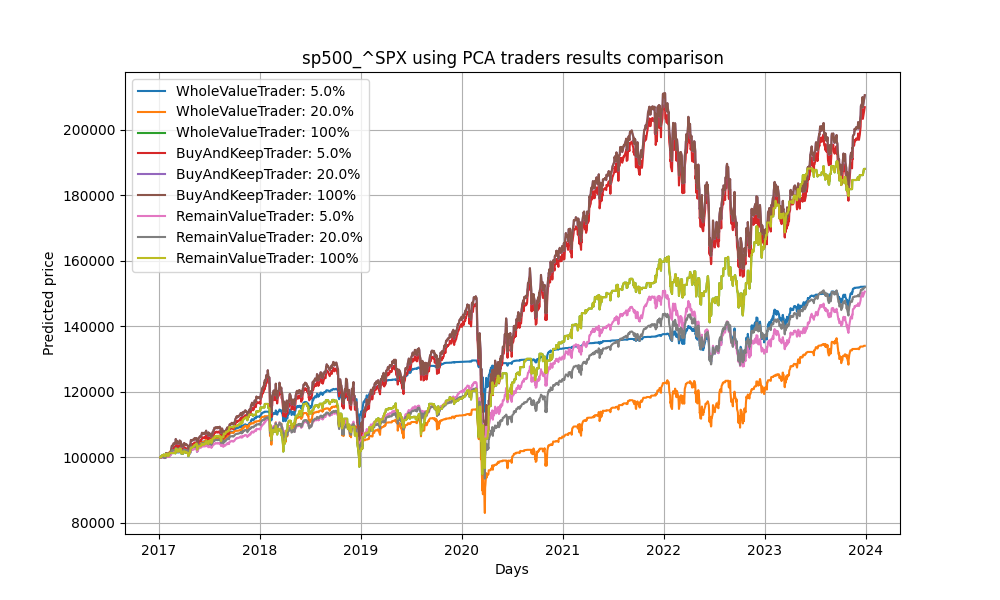
\includegraphics[width=\linewidth]{pca_traders.png}
    \caption{Predicted portfolio value over time for different trader types using PCA.}
    \label{fig:pca_trader_portfolio}
\end{figure}

Notably, in the case of individual stocks, such as Nvidia, traders employing the 100\% Remain Value strategy were able to achieve exceptional results, significantly outperforming the index. For example, the portfolio value for Nvidia doubled relative to the overall market trend. This demonstrates that while broader strategies like Buy and Keep capture general market growth, focused approaches on specific high-performing stocks can yield substantial profits.

\begin{figure}[ht!]
    \centering
    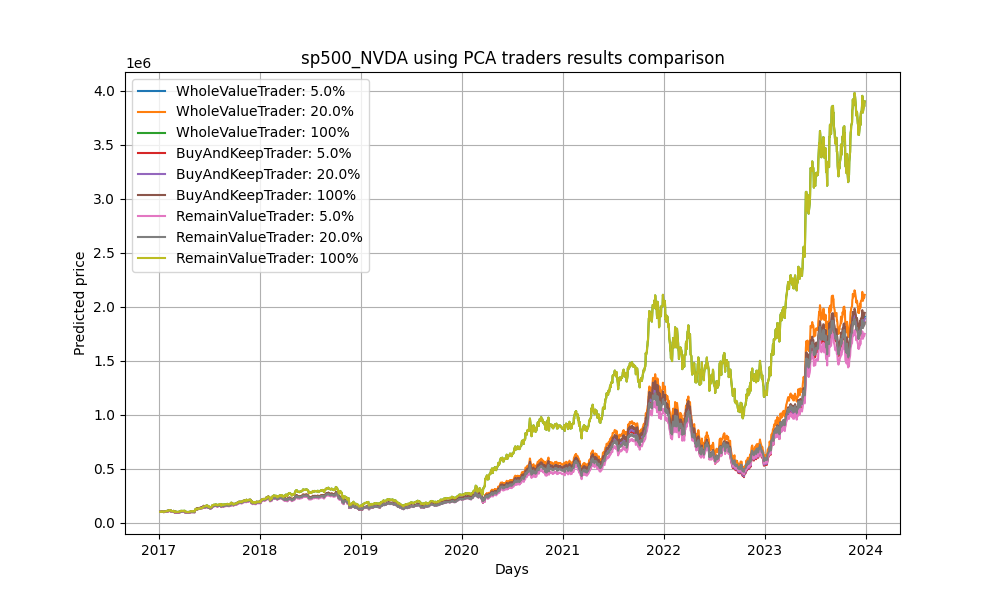
\includegraphics[width=\linewidth]{pca_nvidia_traders.png}
    \caption{Predicted portfolio value over time for Nvidia stock across different trader types using the PCA model.}
    \label{fig:pca_nvidia_trader_portfolio}
\end{figure}

\subsection{Portfolio Value over Time for SVM}

Despite its weak performance in predicting the S\&P 500 index, SVM achieved satisfactory results in the case of individual stocks, such as Chevron Corp. In particular, the Remain Value Trader with a 100\% transaction strategy demonstrated notable success (figure~\ref{fig:cvx_svm_traders}), effectively capitalizing on SVM's accurate short-term predictions for this stock.

\begin{figure}[ht!]
    \centering
    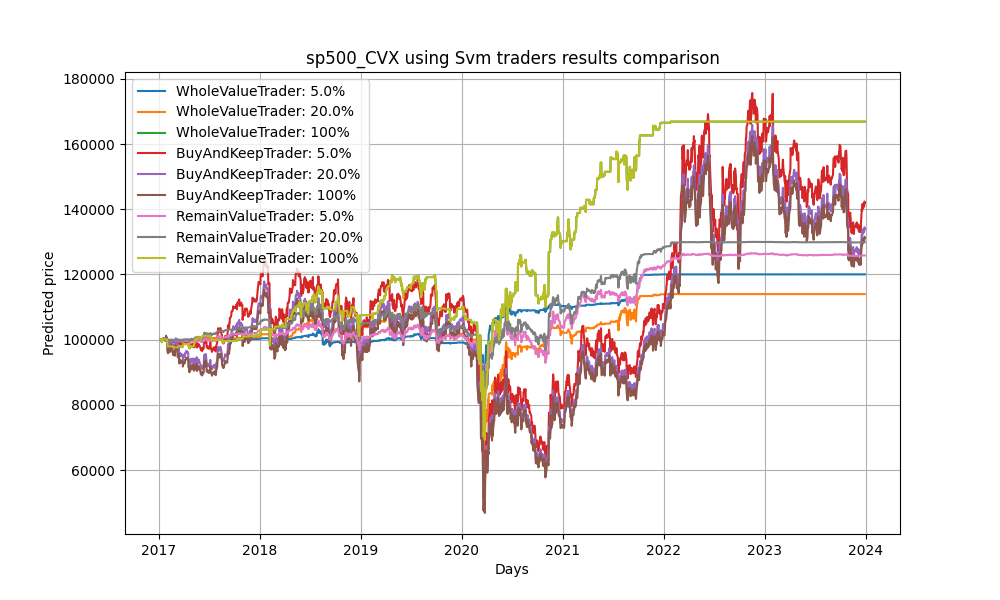
\includegraphics[width=\linewidth]{cvx_svm_traders.png}
    \caption{Predicted portfolio value over time for Chevron Corp stock across different trader types using the SVM model.}
    \label{fig:cvx_svm_traders}
\end{figure}

\subsection{Portfolio Value over Time for QPCA and QSVM}

Unlike the PCA and SVM models, rest of the models show a flat line for all trader types. This outcome is due to the models' predictions being highly erratic and failing to capture meaningful price changes, leading to no buying or selling activity. As a result, the portfolio value remains unchanged throughout the entire test period, reflecting the models' inability to predict price movements effectively.

\section{Conclusions}

\subsection{Prediction performance}

Based on the results of the prediction and error analysis, it is clear that PCA (Principal Component Analysis) outperforms SVM (Support Vector Machine) in predicting stock prices for the S\&P 500 index. PCA demonstrates greater accuracy in tracking the actual index values, despite a slight 1-2 day delay. This highlights its effectiveness in handling stock market data, particularly in volatile market conditions.

The results obtained using SVM show less reliability. There are significant deviations from actual prices, particularly during periods of high market volatility. The SVM model struggles to respond adequately to dynamic price changes, which may stem from its limitations in modeling complex and nonlinear relationships in financial markets.

When incorporating quantum algorithms such as QPCA (Quantum Principal Component Analysis) and QSVM (Quantum Support Vector Machine), the predictions indicate that the quantum approaches currently underperform when compared to their classical counterparts. Despite the theoretical advantages offered by quantum computing, such as the potential for handling more complex data structures and faster computations, QPCA and QSVM face challenges in practice. QPCA, for instance, struggles to effectively capture market dynamics and produces predictions that are largely static, providing no significant improvements over PCA. Similarly, QSVM exhibits large deviations in predictions, especially during volatile periods, suggesting that the quantum SVM is sensitive to noise and does not generalize well for financial data.

These results indicate that while quantum algorithms may offer long-term potential, particularly in terms of computational speed and data complexity, they are not yet on par with classical models in their current form. The noise and complexity inherent in financial data, combined with the significant computational resources required for quantum models, present substantial hurdles.

Based on these findings, it can be concluded that PCA is a more suitable method for stock price prediction in the context of the S\&P 500 index, at least with current algorithms and resources. However, further research is needed to assess the applicability of these findings to other indices and market conditions. Additionally, the introduction of quantum algorithms, such as QPCA and QSVM, may provide further insights and improvements in stock price prediction accuracy, provided that issues related to noise, computational resources, and model refinement are addressed in future developments.

\subsection{Trader Strategy Performance}

From the results, it is clear that the \textit{Buy and Keep Trader} strategy performs the best under the PCA model, followed by the \textit{Remain Value Trader} with a 100\% allocation. The portfolio value for these traders steadily increases, reflecting the overall market trends captured by the PCA model. In contrast, in most scenarios the SVM model fails to provide any meaningful predictions for portfolio growth, as evidenced by the flat portfolio value for all trader types. However, it is worth noting that SVM occasionally demonstrates strong predictive performance, indicating that it may have untapped potential in certain market conditions or specific scenarios.

The introduction of quantum algorithms, such as QPCA and QSVM, raises further questions about their potential impact on trader strategy simulations. The results for quantum models show that both QPCA and QSVM struggle to provide reliable predictions, with substantial deviations from actual market trends. As a result, their performance in simulating trader behavior is significantly worse than that of classical models like PCA. While quantum algorithms theoretically offer superior computational power, their current implementations exhibit high sensitivity to noise and other practical challenges, making them less effective for real-world applications in stock market prediction and trading strategy simulation.

\begin{thebibliography}{99}

\bibitem{pca} 
Jolliffe, I. T. (2002). \textit{Principal Component Analysis}. Springer. \url{https://doi.org/10.1007/b98835}

\bibitem{svm} 
Cortes, C., \& Vapnik, V. (1995). Support-vector networks. \textit{Machine Learning}, 20(3), 273–297. \url{https://doi.org/10.1007/BF00994018}

\bibitem{qpca} 
Lloyd, S., Mohseni, M., \& Rebentrost, P. (2014). Quantum principal component analysis. \textit{Nature Physics}, 10, 631–633. \url{https://doi.org/10.1038/nphys3029}

\bibitem{qsvm} 
Rebentrost, P., Mohseni, M., \& Lloyd, S. (2014). Quantum Support Vector Machine for Big Data Classification. \textit{Physical Review Letters}, 113(13), 130503. \url{https://doi.org/10.1103/PhysRevLett.113.130503}

\bibitem{svm_arxiv} 
Ray, A., Guddanti, S. S., Ajith, V., \& Vinayagamurthy, D. (2022). \textit{Classical ensemble of Quantum-classical ML algorithms for Phishing detection in Ethereum transaction networks}. arXiv:2211.00004v1. \url{https://arxiv.org/abs/2211.00004}

\bibitem{pca_qpca_arxiv} 
Martin, A., Candelas, B., Rodríguez-Rozas, Á., Martín-Guerrero, J. D., Chen, X., Lamata, L., Orús, R., Solano, E., \& Sanz, M. (2019). \textit{Towards Pricing Financial Derivatives with an IBM Quantum Computer}. arXiv:1904.05803v1. \url{https://arxiv.org/abs/1904.05803}

\bibitem{survey_arxiv} 
Author(s). (2024). \textit{Survey of algorithmic trading methods}. arXiv:2405.10119v1. \url{https://arxiv.org/abs/2405.10119}

\bibitem{svm_trading_example} 
Blokker, E. (2008). \textit{The Application of SVM to Algorithmic Trading}. Retrieved from \url{https://cs229.stanford.edu/proj2008/Blokker-TheApplicationofSVMtoAlgorithmicTrading.pdf}

\end{thebibliography}

\end{document}
